
\subsection{Power Supply}
The power supply has been build to deliver three different voltage levels (5V, 6V, 12V), ensuring a current of 1A, 1.5A and 1A respectively.

This circuit has been printed in a PCB that can be plugged directly in a breadboard to deliver the required voltage and current.
The schematics of such can be seen in figure \ref{fig:powersupply_schematics}.

\begin{figure}[H]
\centering 
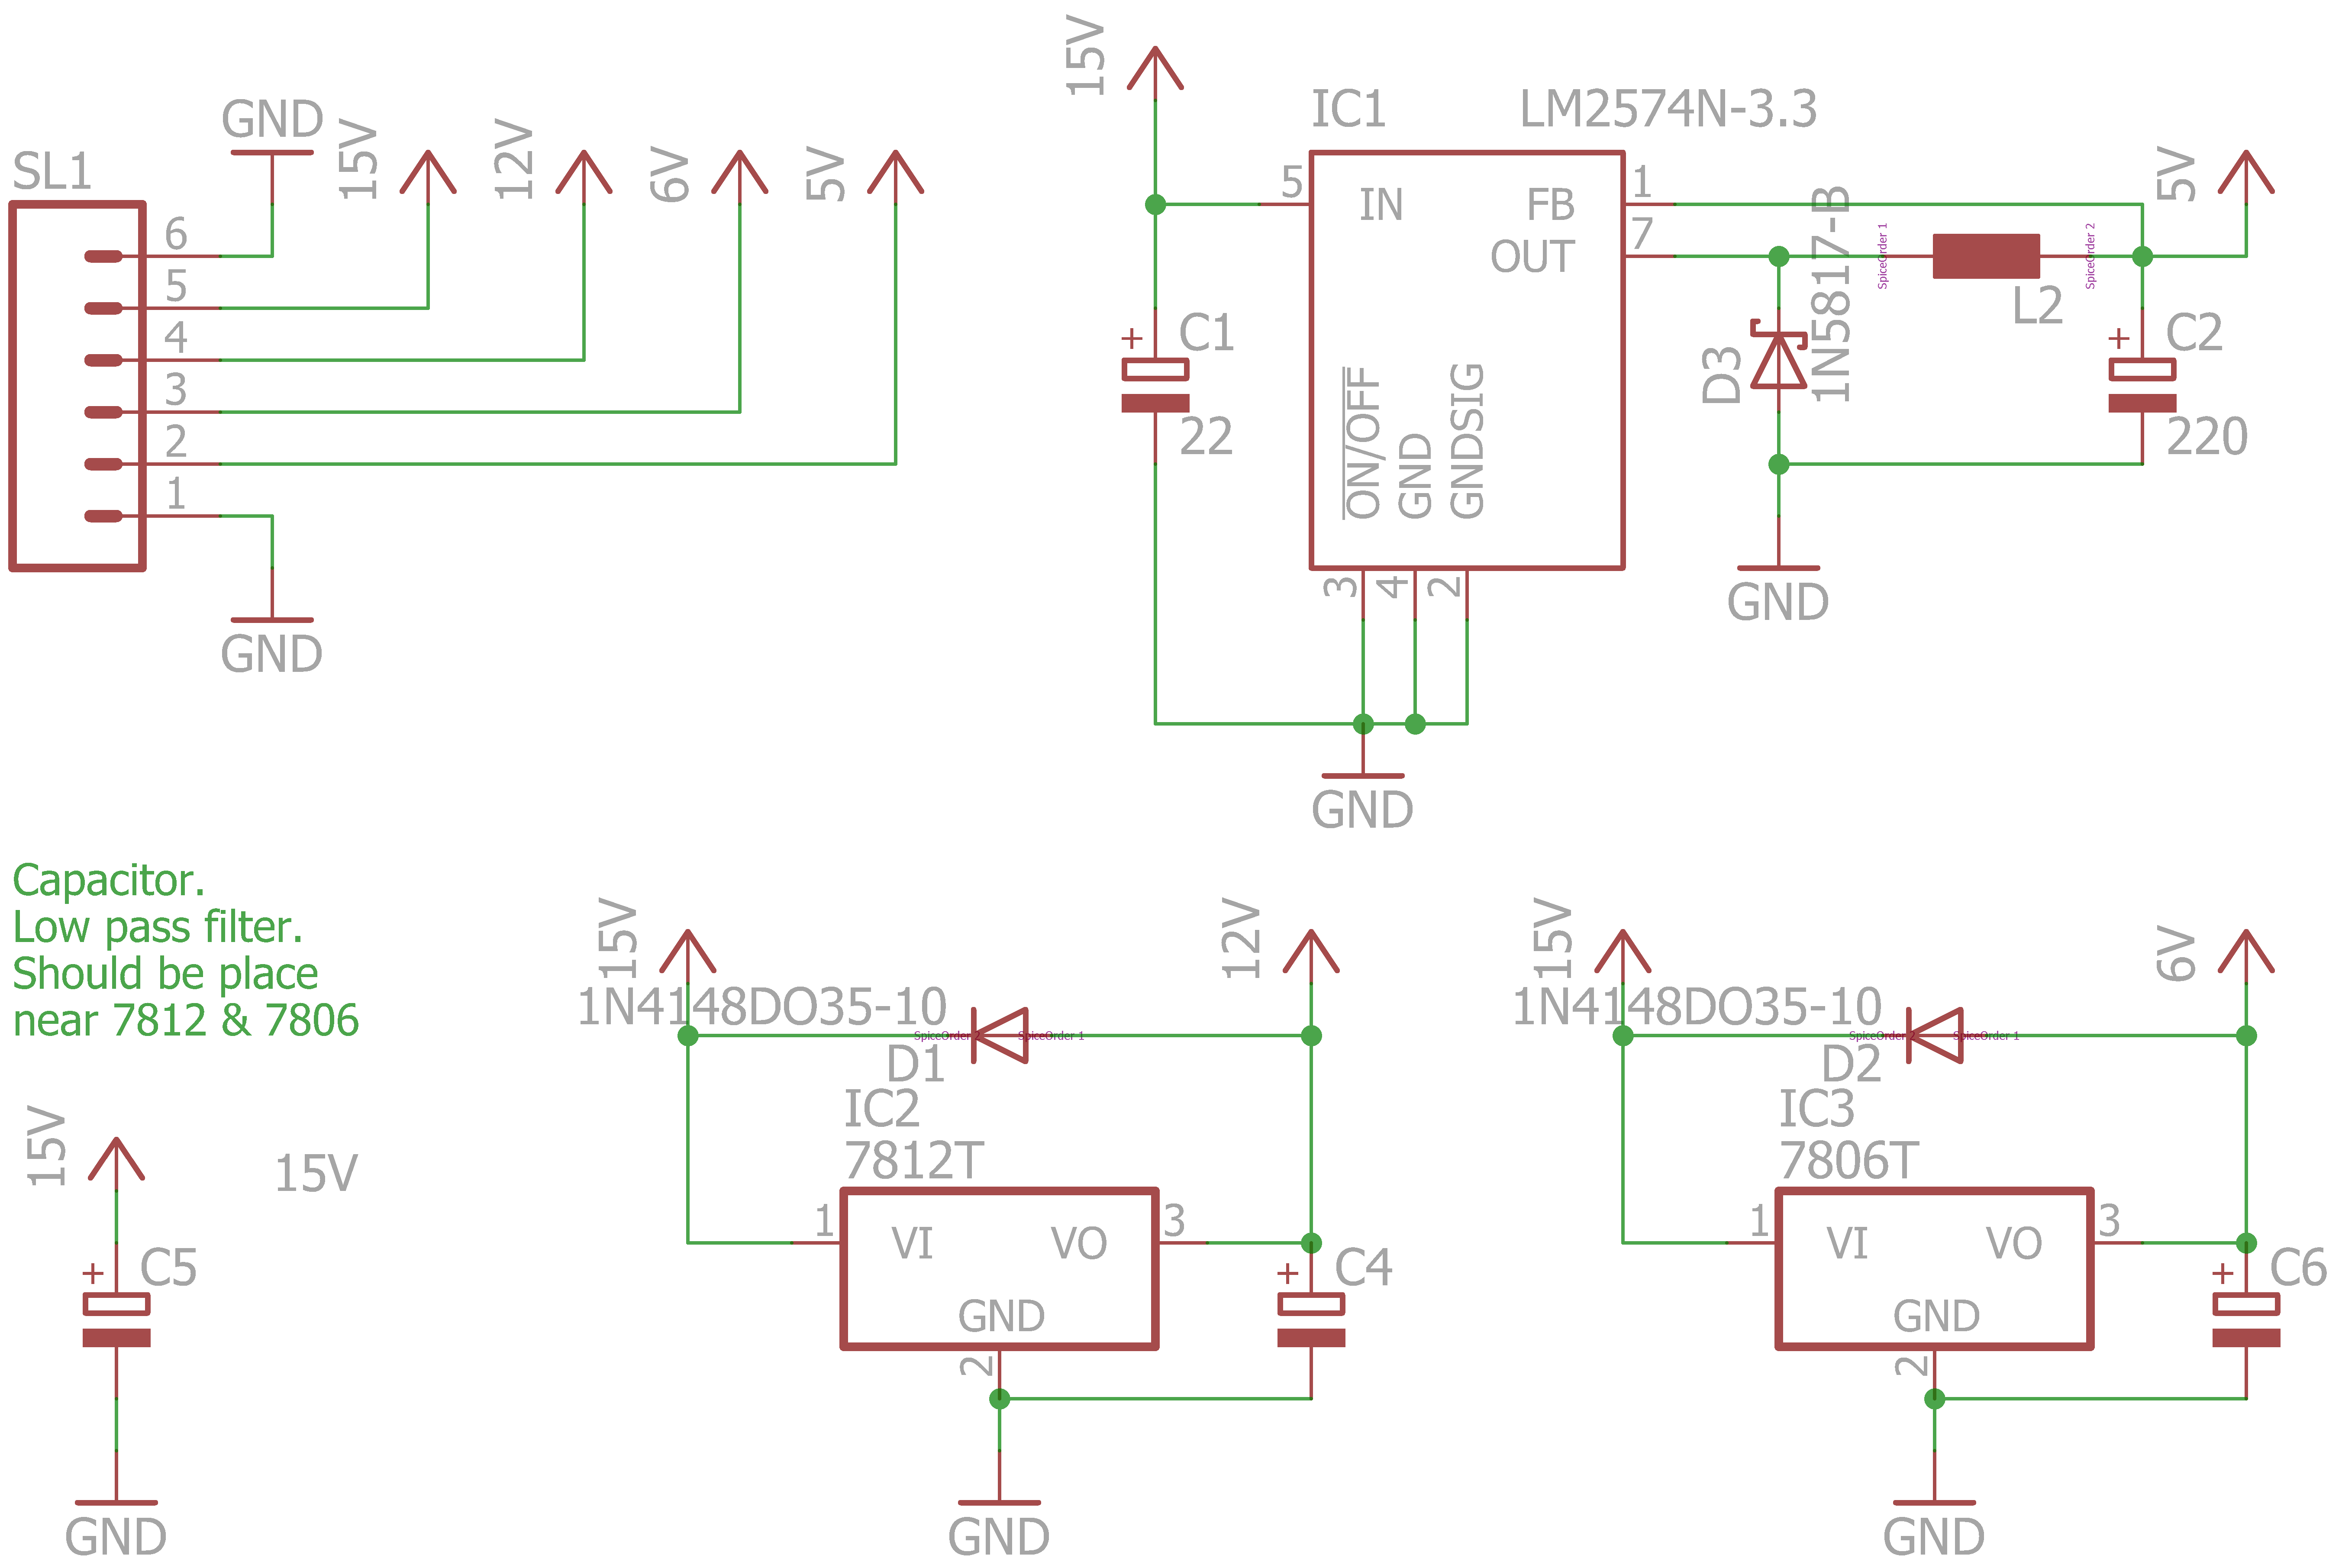
\includegraphics[width = 0.4 \textwidth]{images/powersupply_schematics}
\caption{Schematics of the power supply.}
\label{fig:powersupply_schematics}
\end{figure}


The power supply is connected to a 15V power supply as a input voltage. 
To convert this 15V into 12V, 6V and 5V three different elements are used.
To ensure a 5V/1A supply with a $\pm 1.5\%$ voltage for the FPGA, an LM2574 regulator is used. 
For the 6V/1.5A and 12V/1A, the 7806 and 7812 regulators are used. 
As the efficiency of these regulators is not as good as the one of the LM2574 and they dissipate the excess of power by heating up, a heat-sink for these is required.

The 7806 and 7812 both have a working temperature of maximum $125^{\circ} C$.
In order to hold the temperature of the voltage regulators below this, a heat sink able to dissipate all the heat at the maximum supply rates should be used.

The total energy dissipated by the two regulators can be found by equation \ref{eq:powersupply_energy_dissipation}.

\begin{equation}
P = V_{7806} \cdot I_{7806} + V_{7812} \cdot I_{7812} = (15 - 6) \cdot 1.5 + (15 - 12) \cdot 1 = 16.5W
\label{eq:powersupply_energy_dissipation}
\end{equation}


Estimating the surrounding temperatures to be around $25^{\circ} C$, then the heat sink must keep the temperature below $100^{\circ} C$ when $21W$ is dissipated.
This results in a heat sink capable of rising less than $6 ^{\circ}K per W$ is needed to cool the two regulators.
The \textit{Heatsink SK68 100mm 3K/W TO220} was chosen to do this.
With a $3^{\circ}K/W$ heating coefficient it should be capable of keeping the two regulators at $75^{\circ}C$ during operation with the full load and at a $25^{\circ}c$ ambient temperature.



To test the three power supplies, different load was added to the outputs of the supplies to check if they meet the specified requirements.
The voltage supplied by the regulators was measured by an oscilloscope and the min, max and average recorded for the given load.
The results are seen in table \ref{tab:voltagesupply}.

\begin{table}[H]	
\centering
\begin{tabular}{|c|c|c|c|c|}
\hline
Voltage Supply & Load ($\Omega$) & Min (V) & Avg. (V) & Max (V) \\ \hline
5V & 5 & 4.7167 & 4.7736 & 4.883 \\ \hline
5V & 7.5 & 4.8833 & 5.0496 & 5.05 \\ \hline
5V & 15 & 5.05 & 5.078 & 5.3833 \\ \hline
5V & 33 & 5.05 & 5.1149 & 5.3833 \\ \hline
6V & 4 & 6.05 & 6.1955 & 6.3833 \\ \hline
6V & 7.5 & 6.05 & 6.2163 & 6.3833 \\ \hline
6V & 15 & 6.05 & 6.2183 & 6.3833 \\ \hline
12V & 11 & 11.8833 & 12.0501 & 12.2167 \\ \hline
12V & 16.5 & 12.05 & 12.1835 & 12.2167 \\ \hline
12V & 33 & 12.05 & 12.2137 & 12.3833 \\ \hline
\end{tabular}
\caption{Voltage output table of the voltage regulators using different loads.}
\label{tab:voltagesupply}
\end{table}

\todo[inline]{make this to a V vs I graph with the 3 supplies}


As seen in table \ref{tab:voltagesupply} then the power supplies supply a voltage slightly less than desired when exposed to the full load, but as this decreases the voltage reaches the desired voltage.
This might not be desirable, but it is deemed good enough for the project since the power supply rarely will be used at with full load.


Furthermore the efficiency of the 5V power supply was calculated.
This was done using equation \ref{eq:powersupply_efficiency}.

\begin{equation}
Efficiency = \frac{P_{out}}{P_{in}} = \frac{V_{out}^2 / R_{out}}{V_{in} \cdot I_{in}}
\label{eq:powersupply_efficiency}
\end{equation}

Where, in equation \ref{eq:powersupply_efficiency}, V is the voltage (V), R the load ($\Omega$) and I the current (A) for the circuit where \textit{in} is what was supplied by the 15V supply and \textit{out} the output of the regulator.


\begin{table}[H]
\centering
\begin{tabular}{|c|c|c|c|c|}
\hline
Load ($\Omega$) & Min Efficiency & Avg. Efficiency & Max Efficiency \\ \hline
5 & 0.7806 & 0.7996 & 0.8367 \\ \hline
7.5 & 0.7570 & 0.8095 & 0.8096 \\ \hline
15 & 0.7556 & 0.7640 & 0.8587 \\ \hline
33 & 0.644 & 0.6607 & 0.7318 \\ \hline
\end{tabular}
\caption{Efficiency of the 5V supply.}
\label{tab:voltageefficiency}
\end{table}